\section{Plot Generation}
Each block that is sent into the plot generator is treated differently depending on what the block label is. 
If the block label is either \textit{Parks} or \textit{Parking}, the entire block is turned into a plot and is sent to the park generator or park generator respectively.
The rest of the block labels are split into multiple parts, where the amount of resulting plots depend on the area of the block as well as some random variables. 

Figure~\ref{fig:plot2} and \ref{fig:plot} demonstrates some example outputs from the plot generator.

\begin{figure}[H]
  \centering

  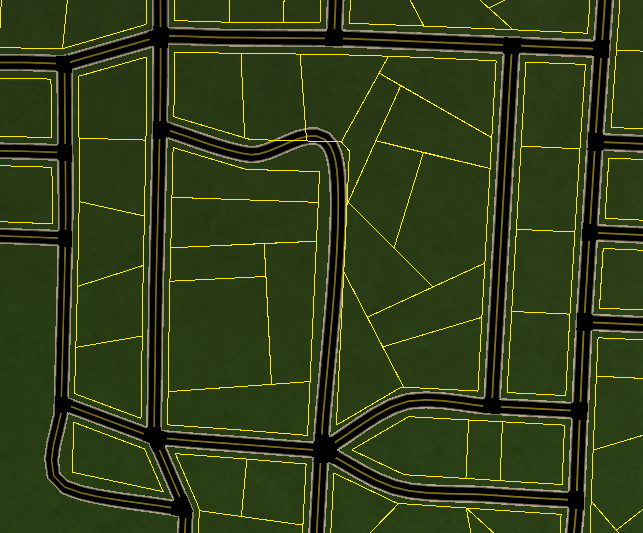
\includegraphics[width=0.8\textwidth]{figure/plot2.png}
  \caption{Close-up of the plot splitting algorithm.}

  \label{fig:plot2}
\end{figure}

\begin{figure}[H]
  \centering

  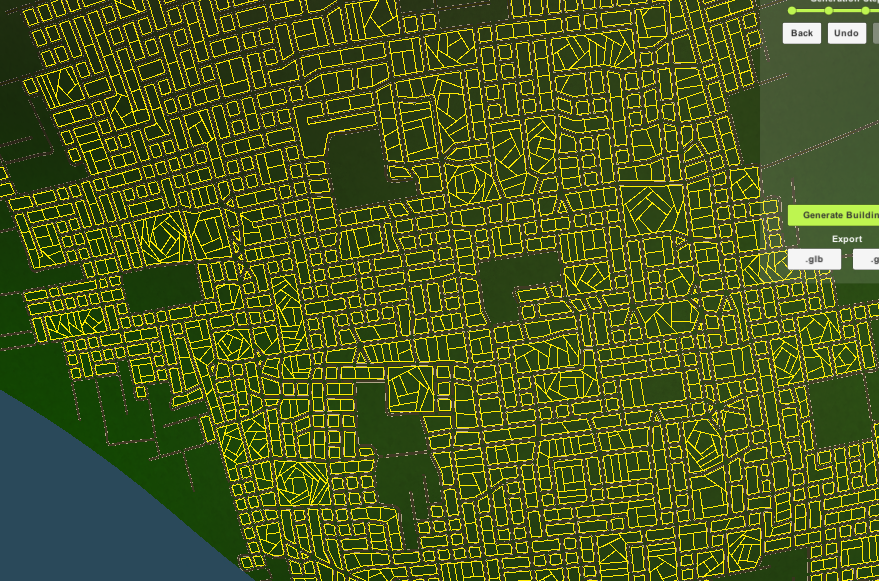
\includegraphics[width=0.8\textwidth]{figure/plot.png}
  \caption{Generated plots within a larger city.}

  \label{fig:plot}
\end{figure}

Each plot is assigned a plot label depending on the size of the plot and the population map.
The plot labels are \textit{Manhattan}, \textit{Skyscraper}, \textit{Park}, \textit{Parking}, and \textit{Empty}.
\textit{Manhattan} and \textit{Skyscraper} are two different sub-generators for building generator. 
\textit{Park} and \textit{Parking} are used by the park generator and the parking generator respectively.
If the plot label is \textit{Empty}, then no content is generated upon the plot.
Larger plots are always assigned with the \textit{Park} label.
The purpose of the plot labels is to let other generators know what should be generated within the plot.